\documentclass[aspectratio=169,12pt,t]{beamer}

% --- Theme: Metropolis (modern, clean) ---
\usetheme[progressbar=frametitle,numbering=fraction,block=fill]{metropolis}

% --- Fira Sans font (install texlive-fonts-extra if missing) ---
\IfFileExists{FiraSans.sty}{\usepackage[sfdefault]{FiraSans}}{}

% --- Light background with warm accent ---
\definecolor{mDarkTeal}{RGB}{35,55,59}
\definecolor{mLightBrown}{RGB}{235,228,216}
\definecolor{mAccent}{RGB}{140,70,20}

\setbeamercolor{normal text}{fg=mDarkTeal,bg=white}
\setbeamercolor{alerted text}{fg=mAccent}
\setbeamercolor{frametitle}{bg=mDarkTeal,fg=white}
\setbeamercolor{progress bar}{fg=mAccent,bg=mLightBrown}
\setbeamercolor{title separator}{fg=mAccent}
\setbeamercolor{progress bar in head/foot}{fg=mAccent,bg=mLightBrown}
\setbeamercolor{progress bar in section page}{fg=mAccent,bg=mLightBrown}

% --- Packages ---
\usepackage[utf8]{inputenc}
\usepackage{amsmath,amssymb,amsthm}
\usepackage{mathrsfs}
\usepackage{tikz}
\usetikzlibrary{arrows.meta,positioning,calc,decorations.pathreplacing,shapes,patterns}
\usetikzlibrary{shadows.blur,backgrounds,fadings}
\usepackage{pgfplots}
\pgfplotsset{compat=1.18}

% --- Shared diagram styling (consistent, polished look across all figures) ---
\tikzset{
  axisln/.style={-{Stealth[length=2.6mm]}, line width=0.8pt, gray!75},
  curveln/.style={line width=1.6pt, line cap=round, line join=round},
  projln/.style={dash pattern=on 2.6pt off 2pt, line width=0.7pt},
  guide/.style={-{Stealth[length=2.6mm,width=2.2mm]}, line width=1.1pt},
}
% soft rounded background panel for inset plots
\tikzset{panel/.style={rounded corners=6pt, draw=mDarkTeal!14, line width=0.8pt,
  fill=mDarkTeal!4,
  blur shadow={shadow blur steps=8, shadow opacity=13,
               shadow xshift=0pt, shadow yshift=-1.3pt}}}
% point marker with a white halo: \dotpt{color}{(coord)}
\newcommand{\dotpt}[2]{%
  \fill[white] #2 circle (3.6pt);
  \fill[#1] #2 circle (2.4pt);
}
% open point marker: \opendot{color}{(coord)}
\newcommand{\opendot}[2]{%
  \fill[white] #2 circle (3.6pt);
  \draw[#1, line width=1.2pt] #2 circle (2.6pt);
}

% --- Semi-transparent white highlight for text on top of background images ---
\usepackage[most]{tcolorbox}

% Inline highlight: \hl{short text}
\newtcbox{\hl}{%
  nobeforeafter, tcbox raise base,
  colback=white, opacityback=0.6,
  colframe=white, opacityframe=0,
  sharp corners, boxsep=2pt, left=3pt, right=3pt, top=2pt, bottom=2pt%
}

% Block highlight: \begin{hlbox} ... \end{hlbox}  (multi-line, paragraphs, itemize)
\newtcolorbox{hlbox}[1][]{%
  enhanced, breakable,
  colback=white, opacityback=0.6,
  colframe=white, opacityframe=0,
  boxsep=3pt, left=6pt, right=6pt, top=4pt, bottom=4pt,
  sharp corners,
  {#1}%
}

% --- Custom colors for content types ---
\definecolor{defcolor}{RGB}{25,85,120}
\definecolor{thmcolor}{RGB}{140,35,35}
\definecolor{proofcolor}{RGB}{35,100,50}
\definecolor{excolor}{RGB}{140,75,10}
\definecolor{remcolor}{RGB}{90,90,90}

% --- Beamer blocks for mathematical content types (semi-transparent) ---
\tcbset{hlblockbase/.style={
  enhanced, breakable,
  coltitle=white, fonttitle=\bfseries,
  opacitybacktitle=0.8, opacityback=0.6,
  opacityframe=0,
  sharp corners,
  boxsep=1pt, left=5pt, right=5pt, top=2pt, bottom=2pt,
  toptitle=1pt, bottomtitle=1pt
}}

\newtcolorbox{defblock}[1]{hlblockbase, title={#1},
  colbacktitle=defcolor, colback=defcolor!15, colframe=defcolor}
\newtcolorbox{thmblock}[1]{hlblockbase, title={#1},
  colbacktitle=thmcolor, colback=thmcolor!15, colframe=thmcolor}
\newtcolorbox{proofblock}[1]{hlblockbase, title={#1},
  colbacktitle=proofcolor, colback=proofcolor!15, colframe=proofcolor}
\newtcolorbox{exblock}[1]{hlblockbase, title={#1},
  colbacktitle=excolor, colback=excolor!15, colframe=excolor}
\newtcolorbox{remblock}[1]{hlblockbase, title={#1},
  colbacktitle=remcolor, colback=remcolor!15, colframe=remcolor}

% --- Metadata ---
\title{Chapter 4: Continuity}
\subtitle{Section: Infinite Limits and Limits at Infinity}
\author{Based on Walter Rudin's \emph{Principles of Mathematical Analysis}}
\date{}

\begin{document}

{
\usebackgroundtemplate{%
  
\includegraphics[width=\paperwidth,height=\paperheight,keepaspectratio=false]{chapter_04_bg_00.png}%
}
\begin{frame}[plain]
  \titlepage
  \note{
    Welcome back to Chapter 4 on continuity. In this final section we extend
    our notion of a limit so that it works in the extended real number system.
    Up to now, when we wrote that "f" of "t" tends to "A" as "t" tends to "x",
    both "A" and "x" were ordinary real numbers. Here we allow either one, or
    both, to be plus infinity or minus infinity. The clever move is to restate
    the whole definition in the language of neighborhoods, which lets a single
    sentence cover every case at once. Let's see how it works.
  }
\end{frame}
}

{
\usebackgroundtemplate{%
  
\includegraphics[width=\paperwidth,height=\paperheight,keepaspectratio=false]{chapter_04_bg_01.png}%
}
\begin{frame}[c]{Outline}
  \begin{center}
    \tableofcontents
  \end{center}
  \note{
    Here is our plan. We start by recalling why we want to reach into the
    extended reals at all. Then we define neighborhoods of plus and minus
    infinity. With that in hand we give one unified definition of a limit
    that covers finite and infinite cases together. Finally we state the
    arithmetic rules for these limits, and note the forbidden combinations
    that are simply not defined. Let's begin with the motivation.
  }
\end{frame}

\section{Motivation}

% --- Build 1/3 ---
\begin{frame}{Why Extend the Limit?}
  \begin{hlbox}
  \begin{itemize}
    \item So far: $f(t) \to A$ as $t \to x$ with $A, x \in \mathbb{R}$
  \end{itemize}
  \end{hlbox}

  \note{
    Let's recall where we stand. Back in Definition 4.1 we explained what it
    means for "f" of "t" to approach a value "A" as "t" approaches a point "x".
    In that original setting both the target "A" and the point "x" were
    ordinary real numbers. The first bullet on the slide records exactly that
    starting point. Now let's ask what is missing.
  }
\end{frame}

% --- Build 2/3 ---
\begin{frame}{Why Extend the Limit?}
  \begin{hlbox}
  \begin{itemize}
    \item So far: $f(t) \to A$ as $t \to x$ with $A, x \in \mathbb{R}$
    \item We often want $x = \pm\infty$ \;or\; $A = \pm\infty$
  \end{itemize}
  \end{hlbox}

  \note{
    In practice we constantly want to talk about behavior at infinity. What
    happens to "f" of "t" as "t" runs off to plus infinity? When does a
    function blow up to plus infinity as "t" approaches a point? The second
    bullet captures these wishes. We want to allow the point "x", or the
    target "A", or both, to be plus infinity or minus infinity. But our old
    definition only knows about real numbers. We need to enlarge it.
  }
\end{frame}

% --- Build 3/3 ---
\begin{frame}{Why Extend the Limit?}
  \begin{hlbox}
  \begin{itemize}
    \item So far: $f(t) \to A$ as $t \to x$ with $A, x \in \mathbb{R}$
    \item We often want $x = \pm\infty$ \;or\; $A = \pm\infty$
    \item \alert{Key idea:} rephrase Definition 4.1 using \emph{neighborhoods}
  \end{itemize}
  \end{hlbox}

  \note{
    Here is the key idea, and it is a beautiful one. Instead of writing a
    separate definition for each case, we rephrase the original Definition 4.1
    purely in the language of neighborhoods. Once "closeness" is expressed as
    "lying inside a neighborhood", we are free to define a neighborhood of
    infinity as well. A single sentence will then handle finite and infinite
    limits together. Let's first remind ourselves what a neighborhood of a
    real number is.
  }
\end{frame}
}

{
\usebackgroundtemplate{%
  
\includegraphics[width=\paperwidth,height=\paperheight,keepaspectratio=false]{chapter_04_bg_02.png}%
}
\section{Neighborhoods of Infinity}

\begin{frame}{Recall: Neighborhood of a Real Number}
  \begin{defblock}{Neighborhood of a real $x$}
    A neighborhood of a real number $x$ is any segment
    \[
      (x - \delta,\; x + \delta), \qquad \delta > 0.
    \]
  \end{defblock}

  \vspace{0.4em}
  \hl{\textbf{Idea:} ``$t$ is close to $x$'' means ``$t$ lies in such a segment.''}

  \note{
    Before extending anything, let's recall the familiar case shown in the
    blue definition block. A neighborhood of a real number "x" is just an open
    segment centered at "x", running from "x" minus delta to "x" plus delta,
    where delta is some positive number. Saying that "t" is close to "x" is the
    same as saying that "t" sits inside one of these segments. The smaller we
    take delta, the closer we force "t" to be. Now we want a similar notion of
    closeness for plus and minus infinity.
  }
\end{frame}

\begin{frame}{Definition 4.32: Neighborhoods of $\pm\infty$}
  \begin{defblock}{Definition 4.32}
    For any real $c$:
    \begin{itemize}
      \item $(c, +\infty) = \{\, x : x > c \,\}$ is a neighborhood of $+\infty$.
      \item $(-\infty, c) = \{\, x : x < c \,\}$ is a neighborhood of $-\infty$.
    \end{itemize}
  \end{defblock}

  \vspace{0.4em}
  \hl{\textbf{Idea:} ``close to $+\infty$'' means ``larger than some cutoff $c$.''}

  \note{
    Here is the new definition. A neighborhood of plus infinity is any ray of
    the form open interval from "c" to plus infinity, that is, the set of all
    real numbers larger than "c". Similarly a neighborhood of minus infinity is
    the set of all real numbers smaller than "c". Think of "c" as a cutoff. To
    be close to plus infinity simply means to be beyond the cutoff, that is,
    bigger than "c". The larger we choose "c", the deeper into the positive
    reals we force the point. This is the perfect analogue of shrinking delta
    in the finite case. Let's picture it.
  }
\end{frame}

\begin{frame}[c]{Picture: Three Kinds of Neighborhood}
  \begin{center}
  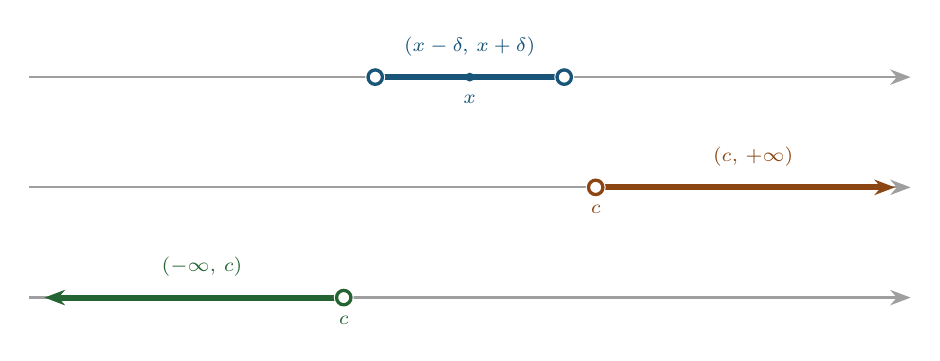
\begin{tikzpicture}[scale=1.0]
    % finite neighborhood
    \draw[axisln] (-5.6,1.4) -- (5.6,1.4);
    \fill[defcolor] (0,1.4) circle (1.6pt) node[below=3pt, font=\scriptsize]{$x$};
    \draw[line width=2.2pt, defcolor] (-1.2,1.4) -- (1.2,1.4);
    \opendot{defcolor}{(-1.2,1.4)} \opendot{defcolor}{(1.2,1.4)}
    \node[defcolor, above=4pt, font=\scriptsize] at (0,1.4) {$(x-\delta,\,x+\delta)$};

    % neighborhood of +infinity
    \draw[axisln] (-5.6,0) -- (5.6,0);
    \fill[mAccent] (1.6,0) circle (1.6pt) node[below=3pt, font=\scriptsize]{$c$};
    \draw[line width=2.2pt, mAccent, -{Stealth[length=2.6mm]}] (1.6,0) -- (5.4,0);
    \opendot{mAccent}{(1.6,0)}
    \node[mAccent, above=4pt, font=\scriptsize] at (3.6,0) {$(c,\,+\infty)$};

    % neighborhood of -infinity
    \draw[axisln] (-5.6,-1.4) -- (5.6,-1.4);
    \fill[proofcolor] (-1.6,-1.4) circle (1.6pt) node[below=3pt, font=\scriptsize]{$c$};
    \draw[line width=2.2pt, proofcolor, -{Stealth[length=2.6mm]}] (-1.6,-1.4) -- (-5.4,-1.4);
    \opendot{proofcolor}{(-1.6,-1.4)}
    \node[proofcolor, above=4pt, font=\scriptsize] at (-3.4,-1.4) {$(-\infty,\,c)$};
  \end{tikzpicture}
  \end{center}

  \note{
    This picture lines up the three kinds of neighborhood. On the top line, in
    blue, is the familiar neighborhood of a real number "x": a bounded segment
    around "x" with open endpoints. On the middle line, in orange, is a
    neighborhood of plus infinity: a ray that starts just past the cutoff "c"
    and shoots off to the right forever, shown by the arrow. On the bottom
    line, in green, is a neighborhood of minus infinity: a ray that starts just
    before "c" and runs off to the left forever. The bounded segment and the
    two unbounded rays now play exactly the same role, which is what lets us
    unify the definition of a limit.
  }
\end{frame}
}

{
\usebackgroundtemplate{%
  
\includegraphics[width=\paperwidth,height=\paperheight,keepaspectratio=false]{chapter_04_bg_03.png}%
}
\section{The Unified Limit}

\begin{frame}{Definition 4.33: Limits in the Extended Reals}
  \begin{defblock}{Definition 4.33}
    Let $f$ be a real function on $E \subset \mathbb{R}$, and let $A, x$ lie in
    the extended reals. We write $f(t) \to A$ as $t \to x$ provided:

    \smallskip
    {\raggedright
    \alert{for every} neighborhood $U$ of $A$,\\
    \alert{there is} a neighborhood $V$ of $x$ with $V \cap E \neq \varnothing$,\\
    \alert{such that}\; $f(t) \in U$ \, for all $t \in V \cap E,\; t \neq x$.\par}
  \end{defblock}

  \note{
    Here is the unified definition, and notice how compact it is. We are given
    a real function "f" on a set "E", and now both the target "A" and the
    approach point "x" may be real or infinite. We say "f" of "t" tends to "A"
    as "t" tends to "x" if the following holds. For every neighborhood "U" of
    the target "A", we can find a neighborhood "V" of the point "x" such that
    "V" actually meets the domain "E", and so that "f" of "t" lands inside "U"
    for every "t" in that overlap, other than "x" itself. Read it slowly: it is
    the usual challenge and response. You hand me a target neighborhood; I must
    supply an approach neighborhood that forces the outputs into your target.
  }
\end{frame}

\begin{frame}{It Agrees with the Old Definition}
  \begin{remblock}{Consistency check}
    When $A$ and $x$ are both \emph{real}, Definition 4.33 says exactly the same
    thing as Definition 4.1.
  \end{remblock}

  \vspace{0.5em}
  \begin{hlbox}
  \begin{itemize}
    \item $U = (A - \varepsilon, A + \varepsilon) \;\Longleftrightarrow\;$ ``$|f(t) - A| < \varepsilon$''
    \item $V = (x - \delta, x + \delta) \;\Longleftrightarrow\;$ ``$0 < |t - x| < \delta$''
  \end{itemize}

  \vspace{0.4em}
  {\footnotesize $\triangleright$\; The strict ``$0 <$'' comes from the clause
  \alert{$t \neq x$}: the limit ignores the value of $f$ \emph{at} $x$.}
  \end{hlbox}

  \note{
    A natural worry: did we change the meaning in the familiar case? The answer
    is no, and the gray block records that reassurance. When both "A" and "x"
    are real, a neighborhood "U" of "A" is just an interval of radius epsilon,
    so the condition "f" of "t" lies in "U" is exactly the statement that the
    distance from "f" of "t" to "A" is less than epsilon. Likewise a
    neighborhood "V" of "x" is an interval of radius delta, so requiring "t" in
    "V" with "t" not equal to "x" is exactly the condition zero less than the
    distance from "t" to "x" less than delta. As the note at the bottom of the
    slide stresses, that strict zero on the left is precisely the requirement
    that "t" is not equal to "x": the limit ignores the value of "f" at "x"
    itself. So the new definition reduces word for word to the old epsilon delta
    definition. Nothing was lost.
  }
\end{frame}

\begin{frame}[c]{Example: $f(t) \to +\infty$ as $t \to 0$}
  \begin{columns}[c]
    \begin{column}{0.52\textwidth}
    \begin{center}
    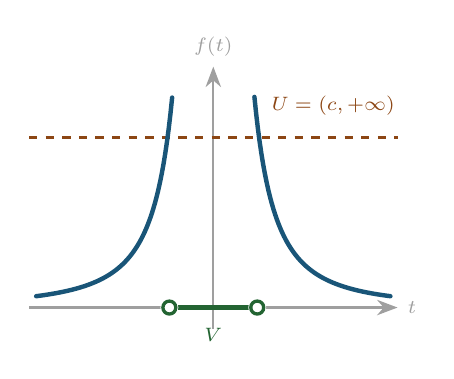
\begin{tikzpicture}[scale=0.9]
      \draw[axisln] (-2.6,0) -- (2.6,0) node[right, font=\scriptsize]{$t$};
      \draw[axisln] (0,-0.3) -- (0,3.4) node[above, font=\scriptsize]{$f(t)$};
      % cutoff line U = (c, +infty)
      \draw[mAccent, dashed, line width=1pt] (-2.6,2.4) -- (2.6,2.4);
      \node[mAccent, font=\scriptsize, anchor=east] at (2.7,2.85) {$U=(c,+\infty)$};
      % curve 1/t^2
      \draw[curveln, defcolor, domain=0.58:2.5, samples=80] plot (\x, {1/(\x*\x)});
      \draw[curveln, defcolor, domain=-2.5:-0.58, samples=80] plot (\x, {1/(\x*\x)});
      % V neighborhood around 0 (open interval: open endpoints)
      \draw[proofcolor, line width=2pt] (-0.62,0) -- (0.62,0);
      \opendot{proofcolor}{(-0.62,0)} \opendot{proofcolor}{(0.62,0)}
      \node[proofcolor, font=\scriptsize, below] at (0,-0.16) {$V$};
    \end{tikzpicture}
    \end{center}
    \end{column}
    \begin{column}{0.46\textwidth}
      \begin{exblock}{$f(t) = 1/t^2$}
        Given any cutoff $c$, choose $\delta$ with
        $1/\delta^2 > c$. Then
        \[
          0 < |t| < \delta \;\Longrightarrow\; f(t) > c.
        \]
        So $f(t) \to +\infty$ as $t \to 0$.
      \end{exblock}
    \end{column}
  \end{columns}

  \note{
    Let's make the infinite case concrete with a picture. The blue curve is the
    graph of "f" of "t" equals one over "t" squared. As "t" approaches zero
    from either side, the curve climbs without bound. Now play the game. Your
    target neighborhood "U" of plus infinity is everything above the orange
    dashed line at height "c". My job is to find an approach neighborhood "V"
    of zero, the green segment on the "t" axis, so that the curve sits above the
    line for every "t" in that segment. Notice the small open circles at the two
    ends of the green segment: they show that "V" is an open interval. And the
    center point zero is left out as well, since the definition only looks at
    "t" different from zero. The amber block shows the choice: pick delta so that
    one over delta squared exceeds "c". Then any nonzero "t" closer than delta
    gives an output above "c". That is precisely "f" of "t" tends to plus
    infinity as "t" tends to zero.
  }
\end{frame}

\begin{frame}[c]{Example: $f(t) \to 0$ as $t \to +\infty$}
  \begin{columns}[c]
    \begin{column}{0.52\textwidth}
    \begin{center}
    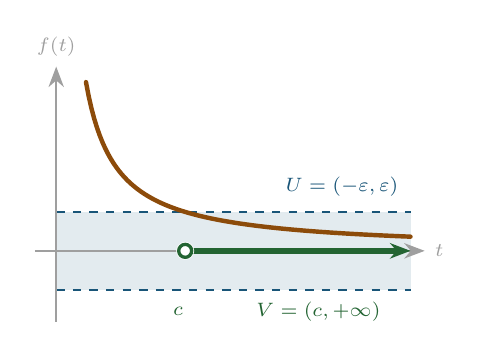
\begin{tikzpicture}[scale=0.9]
      % U = (-eps, eps) band around 0 -- drawn FIRST so the axes sit on top
      \fill[defcolor!12] (0,-0.55) rectangle (5.0,0.55);
      \draw[defcolor, dashed, line width=0.9pt] (0,0.55) -- (5.0,0.55);
      \draw[defcolor, dashed, line width=0.9pt] (0,-0.55) -- (5.0,-0.55);
      % axes (on top of the band)
      \draw[axisln] (-0.3,0) -- (5.2,0) node[right, font=\scriptsize]{$t$};
      \draw[axisln] (0,-1.0) -- (0,2.6) node[above, font=\scriptsize]{$f(t)$};
      \node[defcolor, font=\scriptsize, anchor=west] at (3.1,0.9) {$U=(-\varepsilon,\varepsilon)$};
      % curve 1/t
      \draw[curveln, excolor, domain=0.42:5.0, samples=120] plot (\x, {1/\x});
      % V = (c, +infty) ray on t-axis
      \draw[line width=2.2pt, proofcolor, -{Stealth[length=2.6mm]}] (1.82,0) -- (5.0,0);
      \opendot{proofcolor}{(1.82,0)}
      \node[proofcolor, font=\scriptsize] at (1.72,-0.86) {$c$};
      \node[proofcolor, font=\scriptsize] at (3.7,-0.86) {$V=(c,+\infty)$};
    \end{tikzpicture}
    \end{center}
    \end{column}
    \begin{column}{0.46\textwidth}
      \begin{exblock}{$f(t) = 1/t$ on $(0,\infty)$}
        Given any $\varepsilon > 0$, take the cutoff $c = 1/\varepsilon$.
        Then
        \[
          t > c \;\Longrightarrow\; |f(t)| < \varepsilon.
        \]
        So $f(t) \to 0$ as $t \to +\infty$.
      \end{exblock}
    \end{column}
  \end{columns}

  \note{
    The previous example let the target be infinite. This one lets the approach
    point be infinite, which is the other half of the section title. The amber
    curve is "f" of "t" equals one over "t", and we ask what happens as "t"
    runs off to plus infinity. Now the roles swap. Your target neighborhood "U"
    of zero is the blue band hugging the horizontal axis, stretching from minus
    epsilon up to plus epsilon between the two dashed lines. My approach
    neighborhood "V" of plus infinity is the green ray on the "t" axis,
    everything past a cutoff "c". The amber block shows the choice: take "c"
    equal to one over epsilon. Then for every "t" beyond "c" the curve has
    dropped inside the band, so the size of "f" of "t" is below epsilon. That is
    exactly "f" of "t" tends to zero as "t" tends to plus infinity. Same
    definition, different case.
  }
\end{frame}
}

{
\usebackgroundtemplate{%
  
\includegraphics[width=\paperwidth,height=\paperheight,keepaspectratio=false]{chapter_04_bg_04.png}%
}
\section{Arithmetic of Limits}

\begin{frame}{Theorem 4.34: Limit Arithmetic}
  \begin{thmblock}{Theorem 4.34}
    Let $f, g$ be defined on $E \subset \mathbb{R}$, and suppose
    \[
      f(t) \to A, \qquad g(t) \to B \qquad \text{as } t \to x.
    \]
    Then, \emph{provided the right-hand sides are defined}:
  \end{thmblock}

  \vspace{0.4em}
  \begin{hlbox}
  \begin{itemize}
    \item[(a)] the limit is \alert{unique}: $f(t) \to A'$ implies $A' = A$.
  \end{itemize}
  \end{hlbox}

  \note{
    Now the arithmetic. This is the analogue of Theorem 4.4 from earlier in the
    chapter, and Rudin tells us the proof offers nothing new, so we focus on
    the statement. Suppose "f" of "t" tends to "A" and "g" of "t" tends to "B"
    as "t" tends to "x", where the values may now be infinite. Part "a", shown
    below the red block, is uniqueness: a function cannot approach two different
    limits, so if "f" of "t" also tends to some "A" prime, then "A" prime must
    equal "A". The crucial phrase in the theorem is "provided the right-hand
    sides are defined", and we will see in a moment why that caveat matters.
  }
\end{frame}

\begin{frame}{Theorem 4.34: Limit Arithmetic}
  \begin{thmblock}{Theorem 4.34 (continued)}
    Provided the right-hand sides are defined in the extended reals:
  \end{thmblock}

  \vspace{0.3em}
  \begin{hlbox}
  \begin{itemize}
    \item[(b)] $(f + g)(t) \to A + B$
    \item[(c)] $(fg)(t) \to AB$
    \item[(d)] $(f/g)(t) \to A/B$
  \end{itemize}
  \end{hlbox}

  \note{
    Parts "b", "c", and "d" extend the usual algebra of limits to the extended
    reals. The limit of a sum is the sum of the limits "A" plus "B". The limit
    of a product is the product "A" times "B". And the limit of a quotient is
    the quotient "A" over "B". These look identical to the ordinary rules, and
    that is the point: once we accept the extended arithmetic of plus and minus
    infinity, the same formulas keep working. For instance, if "f" of "t" tends
    to plus infinity while "g" of "t" tends to 5, then the sum tends to plus
    infinity, and the product tends to plus infinity as well. But there is a
    catch built into every line, the words "provided the right-hand sides are
    defined". Let's see what can go wrong.
  }
\end{frame}

\begin{frame}{The Forbidden Forms}
  \begin{remblock}{Note (see Definition 1.23)}
    The following are \alert{not defined} in the extended reals:
    \[
      \infty - \infty, \qquad 0 \cdot \infty, \qquad
      \frac{\infty}{\infty}, \qquad \frac{A}{0}.
    \]
  \end{remblock}

  \vspace{0.4em}
  \hl{Theorem 4.34 applies \emph{only} when the right-hand side avoids these.}

  \note{
    Here are the trouble spots. Infinity minus infinity, zero times infinity,
    infinity divided by infinity, and any number divided by zero are simply not
    assigned a value in the extended real number system. This goes back to
    Definition 1.23, where we set up the extended arithmetic and deliberately
    left these combinations undefined. To see why infinity minus infinity has no
    meaning, picture two functions that both grow without bound: their difference
    could approach any number at all, or nothing in particular, depending
    entirely on how fast each one grows. There is simply no single answer worth
    assigning. So Theorem 4.34 carries the safety clause
    we kept emphasizing: the sum, product, or quotient rule holds only when the
    resulting right-hand side is one of the defined expressions. If you land on
    one of these four forbidden forms, the theorem says nothing, and indeed the
    limit can genuinely fail to exist or take different values. These are the
    classic indeterminate forms you will meet again and again.
  }
\end{frame}
}

{
\usebackgroundtemplate{%
  
\includegraphics[width=\paperwidth,height=\paperheight,keepaspectratio=false]{chapter_04_bg_05.png}%
}
\section{Summary}

% --- Build 1/3 ---
\begin{frame}{Summary}
  \begin{hlbox}
  \textbf{Key takeaways:}
  \begin{itemize}
    \item Neighborhoods of $\pm\infty$: rays $(c, +\infty)$ and $(-\infty, c)$
  \end{itemize}
  \end{hlbox}

  \note{
    Let's gather the main ideas. First, the structural step that made
    everything possible: we defined neighborhoods of plus and minus infinity as
    rays. A neighborhood of plus infinity is everything past a cutoff "c", and a
    neighborhood of minus infinity is everything before a cutoff. These unbounded
    rays play the same role that bounded segments play around a finite point.
  }
\end{frame}

% --- Build 2/3 ---
\begin{frame}{Summary}
  \begin{hlbox}
  \textbf{Key takeaways:}
  \begin{itemize}
    \item Neighborhoods of $\pm\infty$: rays $(c, +\infty)$ and $(-\infty, c)$
    \item One definition (4.33) covers all finite and infinite limits
  \end{itemize}
  \end{hlbox}

  \note{
    Second, with those neighborhoods in hand, Definition 4.33 gave a single
    statement covering every case at once. For every neighborhood of the target
    there is a neighborhood of the approach point that drives the outputs into
    it. When the values are real this reduces exactly to the old epsilon delta
    definition, and when they are infinite it captures blow up and behavior at
    infinity, all in the same breath.
  }
\end{frame}

% --- Build 3/3 ---
\begin{frame}{Summary}
  \begin{hlbox}
  \textbf{Key takeaways:}
  \begin{itemize}
    \item Neighborhoods of $\pm\infty$: rays $(c, +\infty)$ and $(-\infty, c)$
    \item One definition (4.33) covers all finite and infinite limits
    \item Arithmetic (4.34) carries over --- except the \alert{undefined forms}
  \end{itemize}

  \vspace{0.6em}
  \textbf{Coming up next:} Chapter 5 --- Differentiation.
  \end{hlbox}

  \note{
    Third, the algebra of limits in Theorem 4.34 carries over unchanged: sums,
    products, and quotients of limits behave as you would hope, as long as the
    right-hand side avoids the forbidden forms infinity minus infinity, zero
    times infinity, infinity over infinity, and division by zero. That completes
    Chapter 4 on continuity. Next we open Chapter 5 and turn to differentiation,
    where these limit ideas become the engine behind the derivative. See you
    there.
  }
\end{frame}
}

\end{document}
